\documentclass[border=10pt]{standalone}
\usepackage{tikz}
\usetikzlibrary{shapes.geometric, arrows.meta, positioning, calc, fit}
\usepackage[T1]{fontenc}
\usepackage{helvet}
\renewcommand{\familydefault}{\sfdefault}

\begin{document}
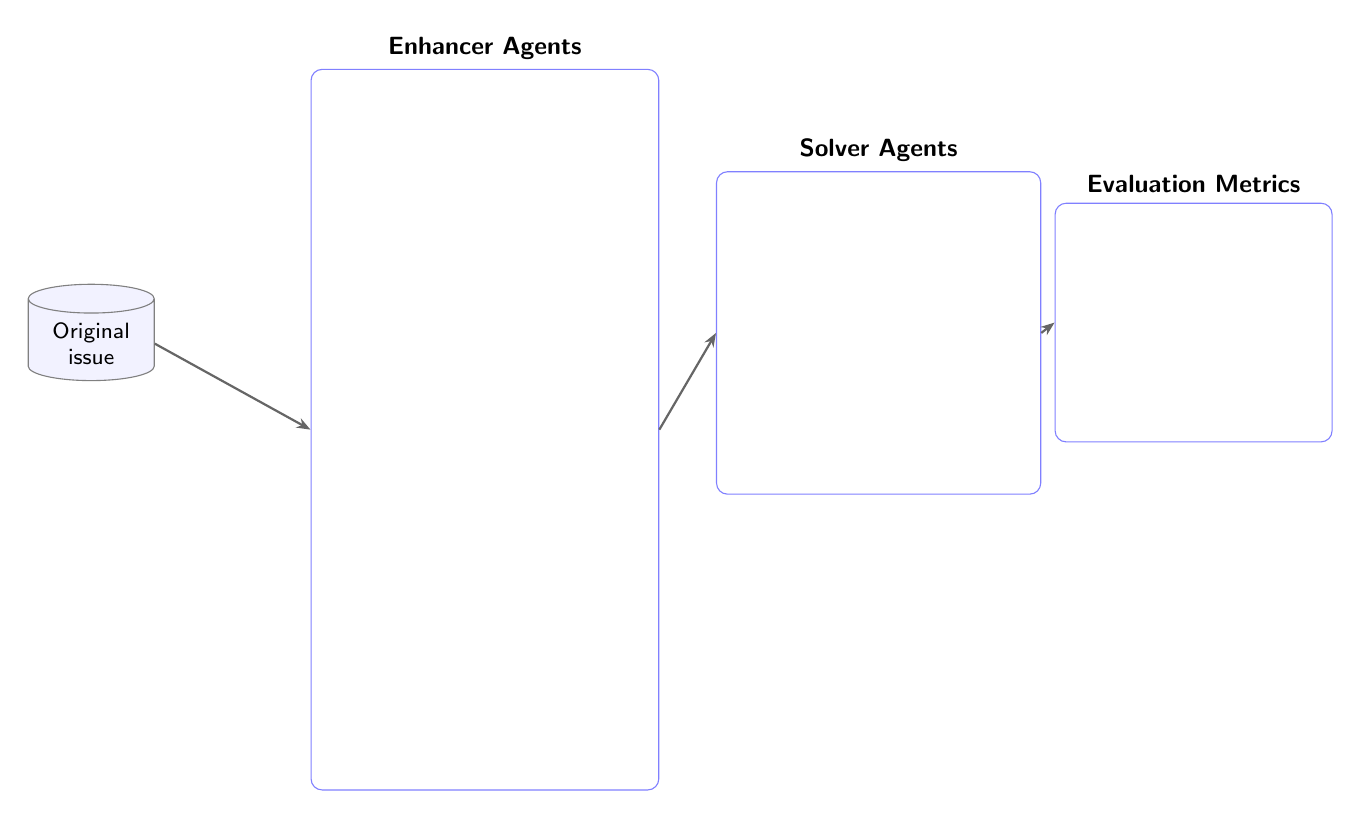
\begin{tikzpicture}[
    node distance=0.4cm,
    agent/.style={rectangle, draw=black!40, fill=blue!8, rounded corners=3pt,
                  minimum height=0.85cm, minimum width=3.4cm, align=center,
                  font=\footnotesize},
    metric/.style={rectangle, draw=black!40, fill=blue!8, rounded corners=3pt,
                   minimum height=0.85cm, minimum width=2.8cm, align=center,
                   font=\footnotesize},
    groupbox/.style={rectangle, draw=blue!50, rounded corners=4pt,
                     inner sep=8pt, fill=white},
    grouplabel/.style={font=\small\bfseries, anchor=south},
    arrow/.style={-{Stealth[length=5pt]}, thick, draw=black!60},
    db/.style={cylinder, draw=black!50, fill=blue!5, shape border rotate=90,
               aspect=0.3, minimum height=1.2cm, minimum width=1.6cm,
               font=\footnotesize, align=center},
]

% Original issue (database icon)
\node[db] (issue) {Original\\issue};

% --- Enhancer Agents ---
\node[agent] (e1) at (5, 2.7)  {No enhancement / Baseline};
\node[agent, below=of e1] (e2) {Raw LLM};
\node[agent, below=of e2] (e3) {Aider};
\node[agent, below=of e3] (e4) {TRAE};
\node[agent, below=of e4] (e5) {OpenHands};
\node[agent, below=of e5] (e6) {SWE-agent};
\node[agent, below=of e6] (e7) {Mini-SWE-agent};

% Group box around enhancers
\node[groupbox, fit=(e1)(e7), inner sep=10pt] (ebox) {};
\node[grouplabel] at (ebox.north) {Enhancer Agents};

% --- Solver Agents ---
\node[agent] (s1) at (10, 1.4)  {Mini-SWE-agent};
\node[agent, below=of s1] (s2) {SWE-agent};
\node[agent, below=of s2] (s3) {Aider};

% Group box around solvers
\node[groupbox, fit=(s1)(s3), inner sep=10pt] (sbox) {};
\node[grouplabel] at (sbox.north) {Solver Agents};

% --- Evaluation Metrics ---
\node[metric] (m1) at (14, 1.0) {Resolved};
\node[metric, below=0.6cm of m1] (m2) {P2P};

% Group box around metrics
\node[groupbox, fit=(m1)(m2), inner sep=10pt] (mbox) {};
\node[grouplabel] at (mbox.north) {Evaluation Metrics};

% --- Arrows ---
% Issue to enhancers
\draw[arrow] (issue.east) -- (ebox.west);

% Enhancers to solvers
\draw[arrow] (ebox.east) -- (sbox.west);

% Solvers to metrics
\draw[arrow] (sbox.east) -- (mbox.west);

\end{tikzpicture}
\end{document}
